\documentclass{beamer}
%\usepackage{ngerman}
\usepackage{inputenc}
\usepackage{listings}
\usepackage[T1]{fontenc}

\definecolor{hilight}{rgb}{.1,.3,.4}
\definecolor{lolight}{rgb}{.7,.7,.7}
\definecolor{ultralolight}{rgb}{.85,.85,.85}
\definecolor{url}{rgb}{.2,.5,.7}
\definecolor{keyword1}{rgb}{.6,.2,.3}
\definecolor{keyword2}{rgb}{.6,.6,.2}
\definecolor{literal}{rgb}{.2,.4,.5}

\setbeamercovered{transparent=0}
\newcommand{\sframe}[1]{\frame{\huge \begin{center} #1 \end{center}}}
\newcommand{\tframe}[2]{\frame{\frametitle{#1}#2}}
\newcommand{\cframe}[2]{\frame{\frametitle{#1}\large \begin{center} #2 \end{center}}}
\newcommand{\hilight}[1]{\textbf{\color{hilight}{#1}}}
\newcommand{\lolight}[1]{\textit{\color{lolight}{#1}}}
\newcommand{\code}[1]{\texttt{#1}}
\renewcommand{\url}[1]{\texttt{\color{url}{#1}}}

\newcommand{\KW}[1]{\color{keyword1}{#1}}
\newcommand{\IKW}[1]{\color{keyword2}{#1}}
\newcommand{\LIT}[1]{\color{literal}{#1}}

\newcommand{\sprod}[2]{\langle #1, #2 \rangle}
\DeclareMathOperator*{\argmax}{arg\,max}
\beamertemplatenavigationsymbolsempty

\title{Game On}
\subtitle{Spiele programmieren mit L�VE}
\author{vrld}
\date{GPN 11}

\mode<presentation>{
	\useoutertheme{shortinfoline}
	\useinnertheme{rounded}
}

\begin{document}

\sframe{
	\Huge \hilight{Game On} \\[.4cm]
	\normalsize
	Spiele programieren mit L�VE \\[.3cm]
	\lolight{GPN 11 // vrld}
}

\sframe{
	\color{ultralolight}{
		\small what is\hspace{6cm}$\,$ \\[.2cm]
		
\includegraphics[width=6cm]{love.png}\\
		\vspace{-.5cm}
		\small \hspace{4cm}... baby don't hurt me
	}
}

\tframe{L�VE}{
	\begin{itemize}
		\item Open Source 2D Game Framework
		\item Lua Scripting
		\item Windows, OSX, Linux (+ Dingoo, Caanoo, OpenPandora)
		\item \url{www.love2d.org}
		\item \url{www.love2d.org/wiki} - Einstiegshilfe
		\item \url{www.love2d.org/forums} - Ausf�hrliche Hilfe
		\item \url{\#love@irc.freenode.net} - Schnelle Hilfe
	\end{itemize}
}

\sframe{
	
\includegraphics[width=6cm]{lua-logo-nolabel.png}
}

\tframe{Lua}{
	\begin{itemize}
		\item Programming in Lua: \url{www.lua.org/pil}
		\item Referenz: \url{www.lua.org/manual/5.1}
		\item Lua Users: \url{lua-users.org/wiki}
		\item Lua Missions: \url{github.com/kikito/lua\_missions}
	\end{itemize}
}

\tframe{Batteries}{
	Wichtig:
	\begin{itemize}
		\item \code{love.graphics}
		\item \code{love.audio}
		\item \code{love.keyboard}, \code{love.mouse}, \code{love.joystick}
	\end{itemize}
	\vspace{.3cm}

	Auch da:
	\begin{itemize}
		\item \code{love.physics}
		\item \code{love.filesystem}
		\item \code{love.thread}
		\item \code{love.sound}
		\item \code{love.timer}
		\item LuaSocket
	\end{itemize}
}

\begin{frame}[fragile]
	\frametitle{Hello, L�VE}
	\color{hilight}{main.lua}\color{black}
	\begin{lstlisting}[escapechar=!]
		!\KW{function}! love.draw()
		    love.graphics.print(!\LIT{"Hello, L�VE"}!, !\LIT{10}!, !\LIT{10}!)
		!\KW{end}!
	\end{lstlisting}
\end{frame}

\tframe{Magnets, ... ?}{
	Running stuff:
	\begin{itemize}
		\item Drag and Drop
		\item \code{love /path/to/game/folder}
		\item \code{love /path/to/game.love}
		\item \code{open -a love /path/to/game[.love]}
	\end{itemize}
	\vspace{.3cm}

	Distributing stuff:
	\begin{itemize}
		\item Umbenannte .zip Datei
		\item \code{main.lua} im top-level
		\item Alles andere egal
	\end{itemize}
}

\begin{frame}[fragile]
	\frametitle{make love \hspace{2cm}\small \color{lolight}\code{make: Nothing to be done for `love'.}\color{black}}
	\scriptsize
	\begin{lstlisting}[escapechar=!]
		!\KW{love}! = /path/to/love
		!\KW{zip}! = /usr/bin/zip
		!\KW{luac}! = /usr/bin/luac

		!\KW{game}! = AWESOMEGAME
		!\KW{sources}! = *.lua */*.lua
		!\KW{res}! = img/*.png snd/*.ogg

		!\IKW{.PHONY}! : run love clean

		!\KW{run}! : test
		    !\KW{\$(love)}! .

		!\KW{test}! : !\KW{\$(sources)}!
		    !\KW{\$(luac)}! !\LIT{-p}! !\KW{\$(sources)}!

		!\KW{love}! : !\KW{\$(game)}!.love

		!\KW{\$(game).love}! : !\KW{\$(sources)}! !\KW{\$(res)}!
		    !\KW{\$(zip)}! !\KW{\$(game)}!!\LIT{.love}! !\KW{\$(sources)}! !\KW{\$(res)}!

		!\KW{clean}! :
		    !\LIT{rm}! !\KW{\$(game)}!!\LIT{.love}!
	\end{lstlisting}
\end{frame}

\cframe{Gameloop}{
	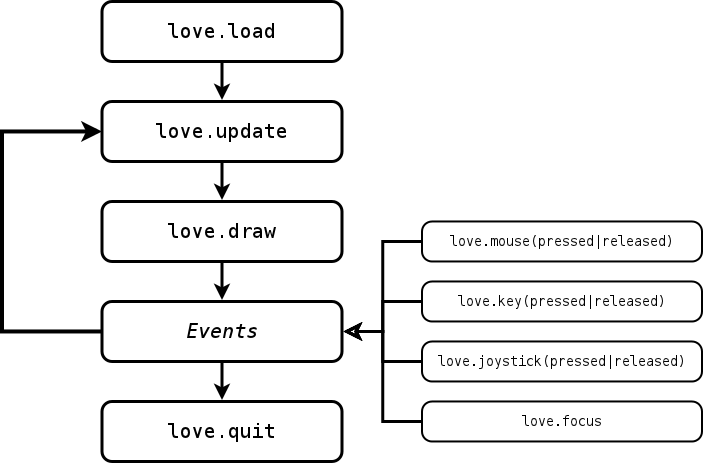
\includegraphics[width=10cm]{gameloop.png}
}

\begin{frame}[fragile]
	\frametitle{Hamsterball}
	\scriptsize
	\begin{lstlisting}[escapechar=!]
!\KW{function}! love.load()
    hamster = {
        img = love.graphics.newImage(!\LIT{'hamster.png'}!),
        x = !\LIT{400}!, y = !\LIT{300}!
    }
!\KW{end}!

!\KW{function}! love.update(dt)
    !\IKW{if}! love.keyboard.isDown(!\LIT{'up'}!) !\IKW{then}!
        hamster.y = hamster.y - dt * !\LIT{100}!
    !\IKW{elseif}! love.keyboard.isDown(!\LIT{'down'}!) !\IKW{then}!
        hamster.y = hamster.y + dt * !\LIT{100}!
    !\IKW{end}!
    !\IKW{if}! love.keyboard.isDown(!\LIT{'left'}!) !\IKW{then}!
        hamster.x = hamster.x - dt * !\LIT{100}!
    !\IKW{elseif}! love.keyboard.isDown(!\LIT{'right'}!) !\IKW{then}!
        hamster.x = hamster.x + dt * !\LIT{100}!
    !\IKW{end}!
!\KW{end}!

!\KW{function}! love.draw()
    love.graphics.draw(hamster.img, hamster.x, hamster.y)
!\KW{end}!
	\end{lstlisting}
\end{frame}

\cframe{Libraries}{
	\begin{itemize}
		\item \hilight{An} \hilight{A}nimation \hilight{L}ibrary \textit{(von bartbes)}
			\begin{itemize}
				\item (Sprite-)Animationen
				\item \url{love2d.org/wiki/AnAL}
			\end{itemize}
		\item LUBE \textit{(von bartbes)}
			\begin{itemize}
				\item LuaSocket wrapper
				\item \url{love2d.org/wiki/LUBE}
			\end{itemize}
		\item MiddleClass und MiddleClass Extras \textit{(von kikito)}
			\begin{itemize}
				\item Klassen-system mit vielen Features
				\item \url{github.com/kikito/MiddleClass}
			\end{itemize}
		\item \hilight{H}elper \hilight{U}tilities for \hilight{M}assive \hilight{P}rogress \textit{(von mir)}
			\begin{itemize}
				\item Gamestates, Timer, Vektoren, Klassen-System, Kamera, Ringbuffer
				\item \url{vrld.github.com/hump}
			\end{itemize}
		\item HardonCollider \textit{(von mir)}
			\begin{itemize}
				\item Kollisionserkennung
				\item \url{vrld.github.com/HardonCollider}
			\end{itemize}
	\end{itemize}
}

\sframe{
	\Huge \hilight{Code On!} \\[.4cm]
}

\end{document}
